% Don't touch this %%%%%%%%%%%%%%%%%%%%%%%%%%%%%%%%%%%%%%%%%%%
\documentclass[12pt]{article}
\usepackage{fullpage}
\usepackage[left=1in,top=1in,right=1in,bottom=1in,headheight=3ex,headsep=3ex]{geometry}
\usepackage{graphicx}
\usepackage{float}
\usepackage{array}


\newcommand{\blankline}{\quad\pagebreak[2]}
%%%%%%%%%%%%%%%%%%%%%%%%%%%%%%%%%%%%%%%%%%%%%%%%%%%%%%%%%%%%%%

% Modify Course title, instructor name, semester here %%%%%%%%

\title{PHY115: Homework 1}
\author{Spring 2021}
\date{}

%%%%%%%%%%%%%%%%%%%%%%%%%%%%%%%%%%%%%%%%%%%%%%%%%%%%%%%%%%%%%%

% Don't touch this %%%%%%%%%%%%%%%%%%%%%%%%%%%%%%%%%%%%%%%%%%%
\usepackage[sc]{mathpazo}
%\linespread{1.05} % Palatino needs more leading (space between lines)
\usepackage[T1]{fontenc}
\usepackage[mmddyyyy]{datetime}% http://ctan.org/pkg/datetime
\usepackage{advdate}% http://ctan.org/pkg/advdate
\newdateformat{syldate}{\twodigit{\THEMONTH}/\twodigit{\THEDAY}}
\newsavebox{\MONDAY}\savebox{\MONDAY}{Mon}% Mon
\newcommand{\week}[1]{%
%  \cleardate{mydate}% Clear date
% \newdate{mydate}{\the\day}{\the\month}{\the\year}% Store date
  \paragraph*{\kern-2ex\quad #1, \syldate{\today} - \AdvanceDate[4]\syldate{\today}:}% Set heading  \quad #1
%  \setbox1=\hbox{\shortdayofweekname{\getdateday{mydate}}{\getdatemonth{mydate}}{\getdateyear{mydate}}}%
  \ifdim\wd1=\wd\MONDAY
    \AdvanceDate[7]
  \else
    \AdvanceDate[7]
  \fi%
}
%\usepackage{setspace}
\usepackage{multicol}
%\usepackage{indentfirst}
\usepackage{fancyhdr,lastpage}
\usepackage{url}
\pagestyle{fancy}
\usepackage{hyperref}
\usepackage{lastpage}
\usepackage{amsmath}
\usepackage{layout}

\lhead{}
\chead{}
%%%%%%%%%%%%%%%%%%%%%%%%%%%%%%%%%%%%%%%%%%%%%%%%%%%%%%%%%%%%%%

% Modify header here %%%%%%%%%%%%%%%%%%%%%%%%%%%%%%%%%%%%%%%%%
%\rhead{\footnotesize Text in header}

%%%%%%%%%%%%%%%%%%%%%%%%%%%%%%%%%%%%%%%%%%%%%%%%%%%%%%%%%%%%%%
% Don't touch this %%%%%%%%%%%%%%%%%%%%%%%%%%%%%%%%%%%%%%%%%%%
\lfoot{}
\cfoot{\small \thepage/\pageref*{LastPage}}
\rfoot{}

\usepackage{array, xcolor}
\usepackage{color,hyperref}
\definecolor{clemsonorange}{HTML}{EA6A20}
\hypersetup{colorlinks,breaklinks,linkcolor=clemsonorange,urlcolor=clemsonorange,anchorcolor=clemsonorange,citecolor=black}

\begin{document}

\maketitle

%\blankline

%\begin{tabular*}{.93\textwidth}{@{\extracolsep{\fill}}lr}

%%%%%%%%%%%%%%%%%%%%%%%%%%%%%%%%%%%%%%%%%%%%%%%%%%%%%%%%%%%%%%


\begin{center}
 Deadline: January 27th    
\end{center}
\hrule



% First Section %%%%%%%%%%%%%%%%%%%%%%%%%%%%%%%%%%%%%%%%%%%%



\section*{Discussion Questions (40 p)}

\begin{enumerate}
  \item Can you have a zero displacement and a nonzero average
  velocity? A nonzero velocity? Illustrate your answers on an $x-t$ graph.
  \item Can you have zero velocity and nonzero average acceleration?
  Zero velocity and nonzero acceleration? Explain using a $v-t$
  graph, and give an example of such motion.
  \item An automobile is traveling west. Can it have a velocity
  toward the west and at the same time have an acceleration toward
  the east? Under what circumstances?
\end{enumerate}


\section*{Exercises (60 p)}


\begin{enumerate}
  \item The fastest measured pitched baseball left
  the pitcher’s hand at a speed of $45~m/s$ If the pitcher was in
  contact with the ball over a distance of $1.5~m$ and produced constant
  acceleration, (a) what acceleration did he give the ball, and
  (b) how much time did it take him to pitch it?
  \item The human body can survive
  an acceleration trauma incident (sudden stop) if the magnitude
  of the acceleration is less than $250~m/s^2$. If you are in an automobile
  accident with an initial speed of $105~km/h$
  and you are stopped by an airbag that inflates from the dashboard,
  over what distance must the airbag stop you for you to survive
  the crash?
\item Two cars, A and B, move
along the x-axis. Figure \ref{1} is
a graph of the positions of A and
B versus time. (a) In motion diagrams, show the position, velocity,
and acceleration of each of
the two cars at $t=0$, $t=1~s$
and $t=3~s$ (b) At what time(s),
if any, do A and B have the same
position? (c) Graph velocity versus
time for both A and B. (d) At what time(s), if any, do A and B
have the same velocity? (e) At what time(s), if any, does car A pass
car B? (f) At what time(s), if any, does car B pass car A?
\end{enumerate}



\begin{figure}[h!]
  
  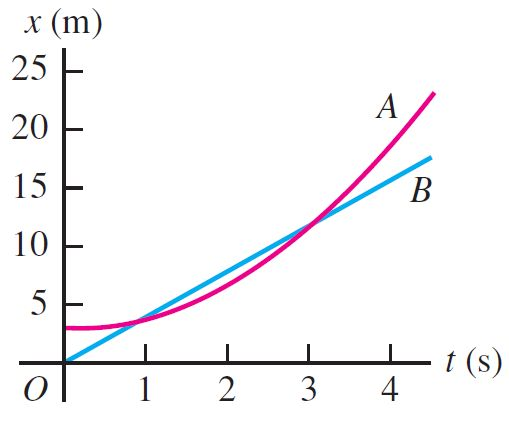
\includegraphics[width=0.65\textwidth]{images/1.jpg}
  \caption{ Position vs. time of two cars. 
  {\tiny © University Physics  with Modern Physics, 13th Edition.} }
  \label{1}
\end{figure}












\end{document}


